\subsection{Error Evaluation}
% \begin{figure*}
%     \begin{minipage}[t]{\columnwidth} % 左側の半分
%         \centering
%         \includegraphics[width=\columnwidth]{fig/reaching_error.pdf}
%         \caption{Length Estimation Error in Reaching Task}
%         \label{fig:reaching_error}
%         \vspace{1em}
%         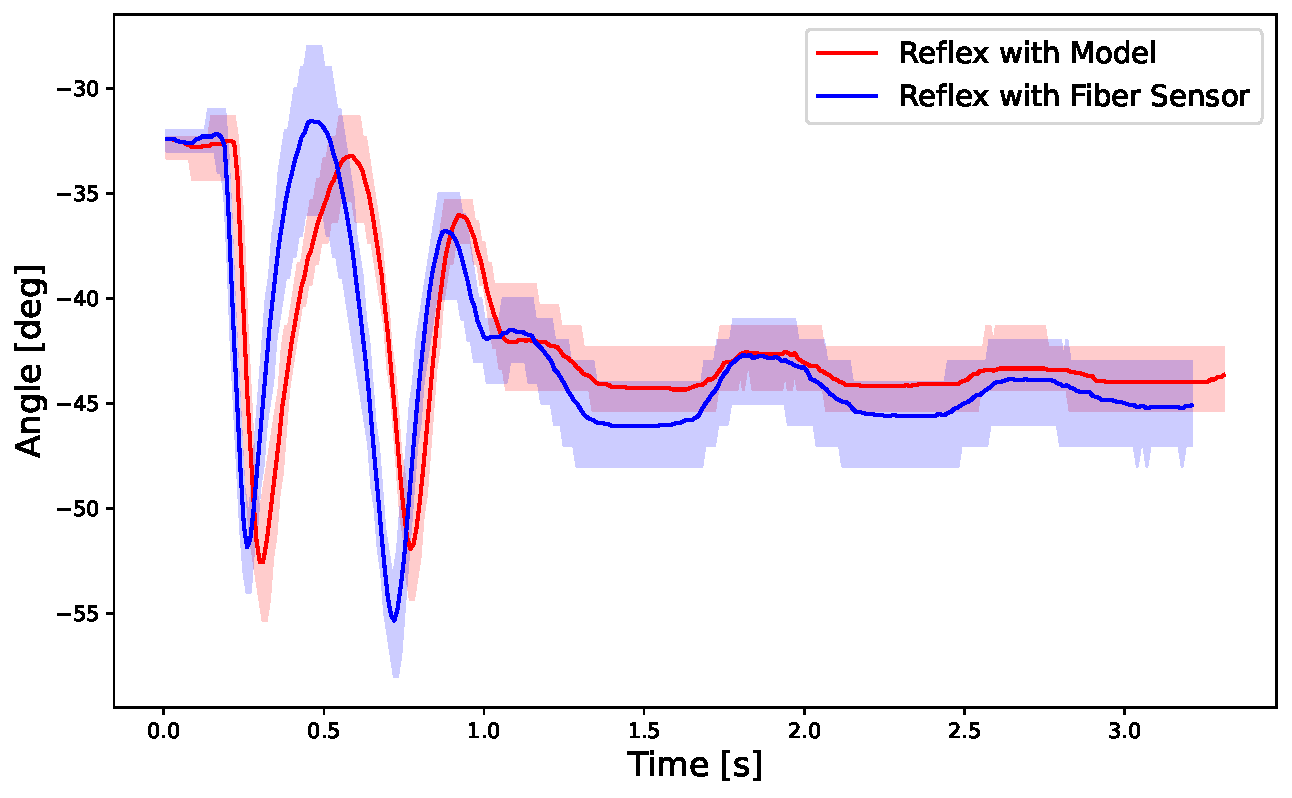
\includegraphics[width=\columnwidth]{fig/time_vs_angle_model_sensor.pdf}
%         \caption{Comparison of Reflex Angles between Model and Fiber Sensor}
%         \label{fig:reflex_angle}
%     \end{minipage}
%     \end{figure*}

% \begin{figure}[t]
%         \centering
%         \includegraphics[width=\columnwidth]{fig/20240819_r20_reflex_all_plt.pdf}
%         \caption{Dynamic Behavior of Reflex by Model}
%         \label{fig:reflex_all}
% \end{figure}


\begin{figure*}[t]
    \centering
    \begin{minipage}[H]{\textwidth} % 全幅を使用
        \begin{minipage}[H]{0.48\textwidth} % 左側の半分
            \centering
            \includegraphics[width=\columnwidth]{fig/reaching_error.pdf}
            \caption{Length Estimation Error in Reaching Task}
            \label{fig:reaching_error}
            \vspace{1em}
            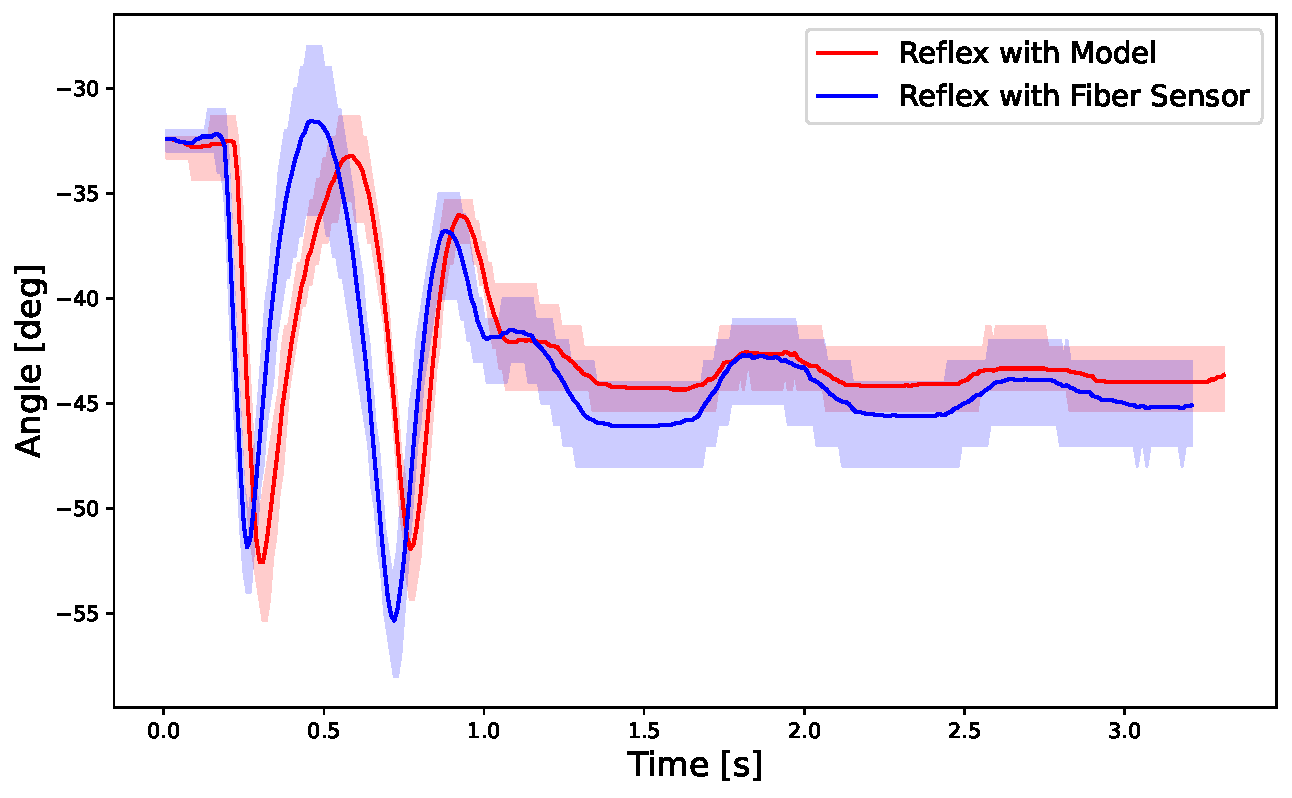
\includegraphics[width=\columnwidth]{fig/time_vs_angle_model_sensor.pdf}
            \caption{Comparison of Reflex Angles between Model and Fiber Sensor}
            \label{fig:reflex_angle}
        \end{minipage}
        \hfill
        \begin{minipage}[H]{0.48\textwidth} % 右側の半分
            \centering
            \includegraphics[width=\columnwidth]{fig/20240819_r20_reflex_all_plt.pdf}
            \caption{Dynamic Behavior of Reflex by Model}
            \label{fig:reflex_all}
        \end{minipage}
    \end{minipage}
\end{figure*}


To improve length estimation accuracy, we expanded Eq. (\ref{eq:model}) by adding the terms $p^2$ and $d^2$ and increasing the parameters as follows:
\begin{equation}
\label{eq:model_2d(1)}
F = (b_5p^2 + b_4pd + b_3d^2 + b_2p+b_1d+b_0)d
\end{equation}
As a result, with respect to the measurements by the linear encoder,the dynamic length estimation was achieved with maximum errors of $1.12\%$ for PAM-A, $0.773\%$ for PAM-B, $1.01\%$ for PAM-B, and $0.755\%$ for PAM-D respectively, and with root mean squared errors of $0.633\%$ for PAM-A, $0.353\%$ for PAM-B, $0.548\%$ for PAM-C, and $0.435\%$ for PAM-D respectively. The errors were reduced as expected for all PAMs. 
% As a result, the dynamic length estimation was achieved with maximum errors within $1.12\%$ and mean squared error rates within $0.633\%$, and the errors were reduced as expected for all PAMs. 

% As a result, as shown in the third and fourth columns of Table \ref{tab:error}, the errors were reduced as expected for all PAMs. 



We also tried another approach by introducing a cubic polynomial model and increasing the parameters as follows:
\begin{equation}
    \label{eq:model_3d}
    F = (c_4p^3+c_3p^2d+c_2pd^2+c_1d^2+c_0)d
\end{equation}
As predicted, the root mean squared errors decreased to $0.516\%$ for PAM-A, $0.484\%$ for PAM-B, $0.500\%$ for PAM-C, and $0.606\%$ for PAM-D respectively. 
However, even though the maximum errors decreased to $1.22\%$ for PAM-A and $0.951\%$ for PAM-C respectively, they actually increased to $1.41\%$ for PAM-B and $1.99\%$ for PAM-D respectively. This result suggests that, even if the coefficients of the model equation are determined experimentally, the degrees must be carefully determined based on previous studies so as to express intrinsic characteristics of the PAM. For example, the newly added term $p^3$ may have amplified the error of the pressure sensor. When applying our model to a reflex mechanism, it will also be necessary to carefully consider the contribution of each term to the accuracy of the length estimation based on the reliability of the force and pressure sensors used.


Wickramatunge et al. proposed separating the parameters $a_i$ into contraction ones $a^c_i$ and extension ones $a^e_i$ to reflect the hysteresis of the PAM\cite{spring}. They also suggested using different parameters for low-pressure and high-pressure ranges to further improve the accuracy. However, our model did not adopt these suggestions and simplifies the length estimation method by using the same parameters across the entire pressure range, regardless of contraction or expansion. This is because our model is supposed to be applied to the reflex mechanism. If the parameters have to be switched depending on the situation, it would be difficult for the reflex mechanism to respond quickly to disturbances.Musculoskeletal robots often carry microcomputers on their structures, so the employed length estimation method is desired to be simple for efficient operation given the limited computational resources.



\subsection{Reaching task}
The maximum errors and the root mean squared errors of the model greatly increased in the reaching task compared to those in the dynamic length estimation in the previous section. One possible cause lies in the process of converting the strain gauge voltage to force. The voltage values fluctuated significantly due to slight positional sift of the fishing line, and the error in the slope of voltage to force $q$ might be amplified during the estimation procedure. Another cause is that as the PAM contracts, the fishing line loses contact with the shaft,resulting in slackness and failure to send voltage signals. In Fig.\ref{fig:reaching_error}, the rate of change in the length estimate by the model decreases at around 3 second because the fishing line loses contact with the shaft and the deformation is estimated as zero from this point onward. This phenomenon poses a disadvantage for continuously tracking the total length of the PAM, but it contributes to creating more biologically inspired behavior. In the human body, a muscle spindle is aligned parallel to a muscle and monitors change in its length, but when the muscle contacts, the muscle spindle becomes unloaded, leading to the cessation of neural discharging activity\cite{spindle}. One of the ultimate goals of our research is to propose a possible operating principle of the reflex mechanism in the human body by incorporating it into a musculoskeletal robot. Our length estimation method is designed in pursuit of this purpose, so it is desirable to develop a local control system that only responds when the muscle is suddenly stretched just as the human neural system does. In this sense, the error during muscle contraction does not need to be a primary concern.


\subsection{Stretch Reflex}
センサーはPAMの直径変化をダイレクトに測ることができるので、インパクトをスパイク状に捉えることができる一方で、モデルは圧力センサの誤差や歪センサの誤差を拾ってしまってlengthの値が大きく揺れ動くので、結果的にVの閾値も大きくなりがちだし、インパクトを明確に分離することができていないので、よりreflexのキャリブレーションが難しい。

Ib反射用にtension sensorhはどうせいるので、センサをまとめられるのは利点。



